\subsection{Installation}
Im Lieferumfang bekommen Sie
\begin{itemize}  
\item gradeplus-0.1.war
\item payara-4.1.2.181.zip
\end{itemize}
Was kommt noch in den Lieferumfang?
\subsubsection{Instruktionen zur Installation}
Client und Server\\
\\
Über die Webseite http://localhost:8080/gradeplus/ kann Grade+ nun geöffnet werden.\\
\\
Auf der Startseite müssten Sie nach aufrufen der Webseite den Login-Bereich sehen (Abbildung \ref{fig 1}).
\begin{figure}[H]
	\centering
	\caption{Startseite und Login-Bereich}
  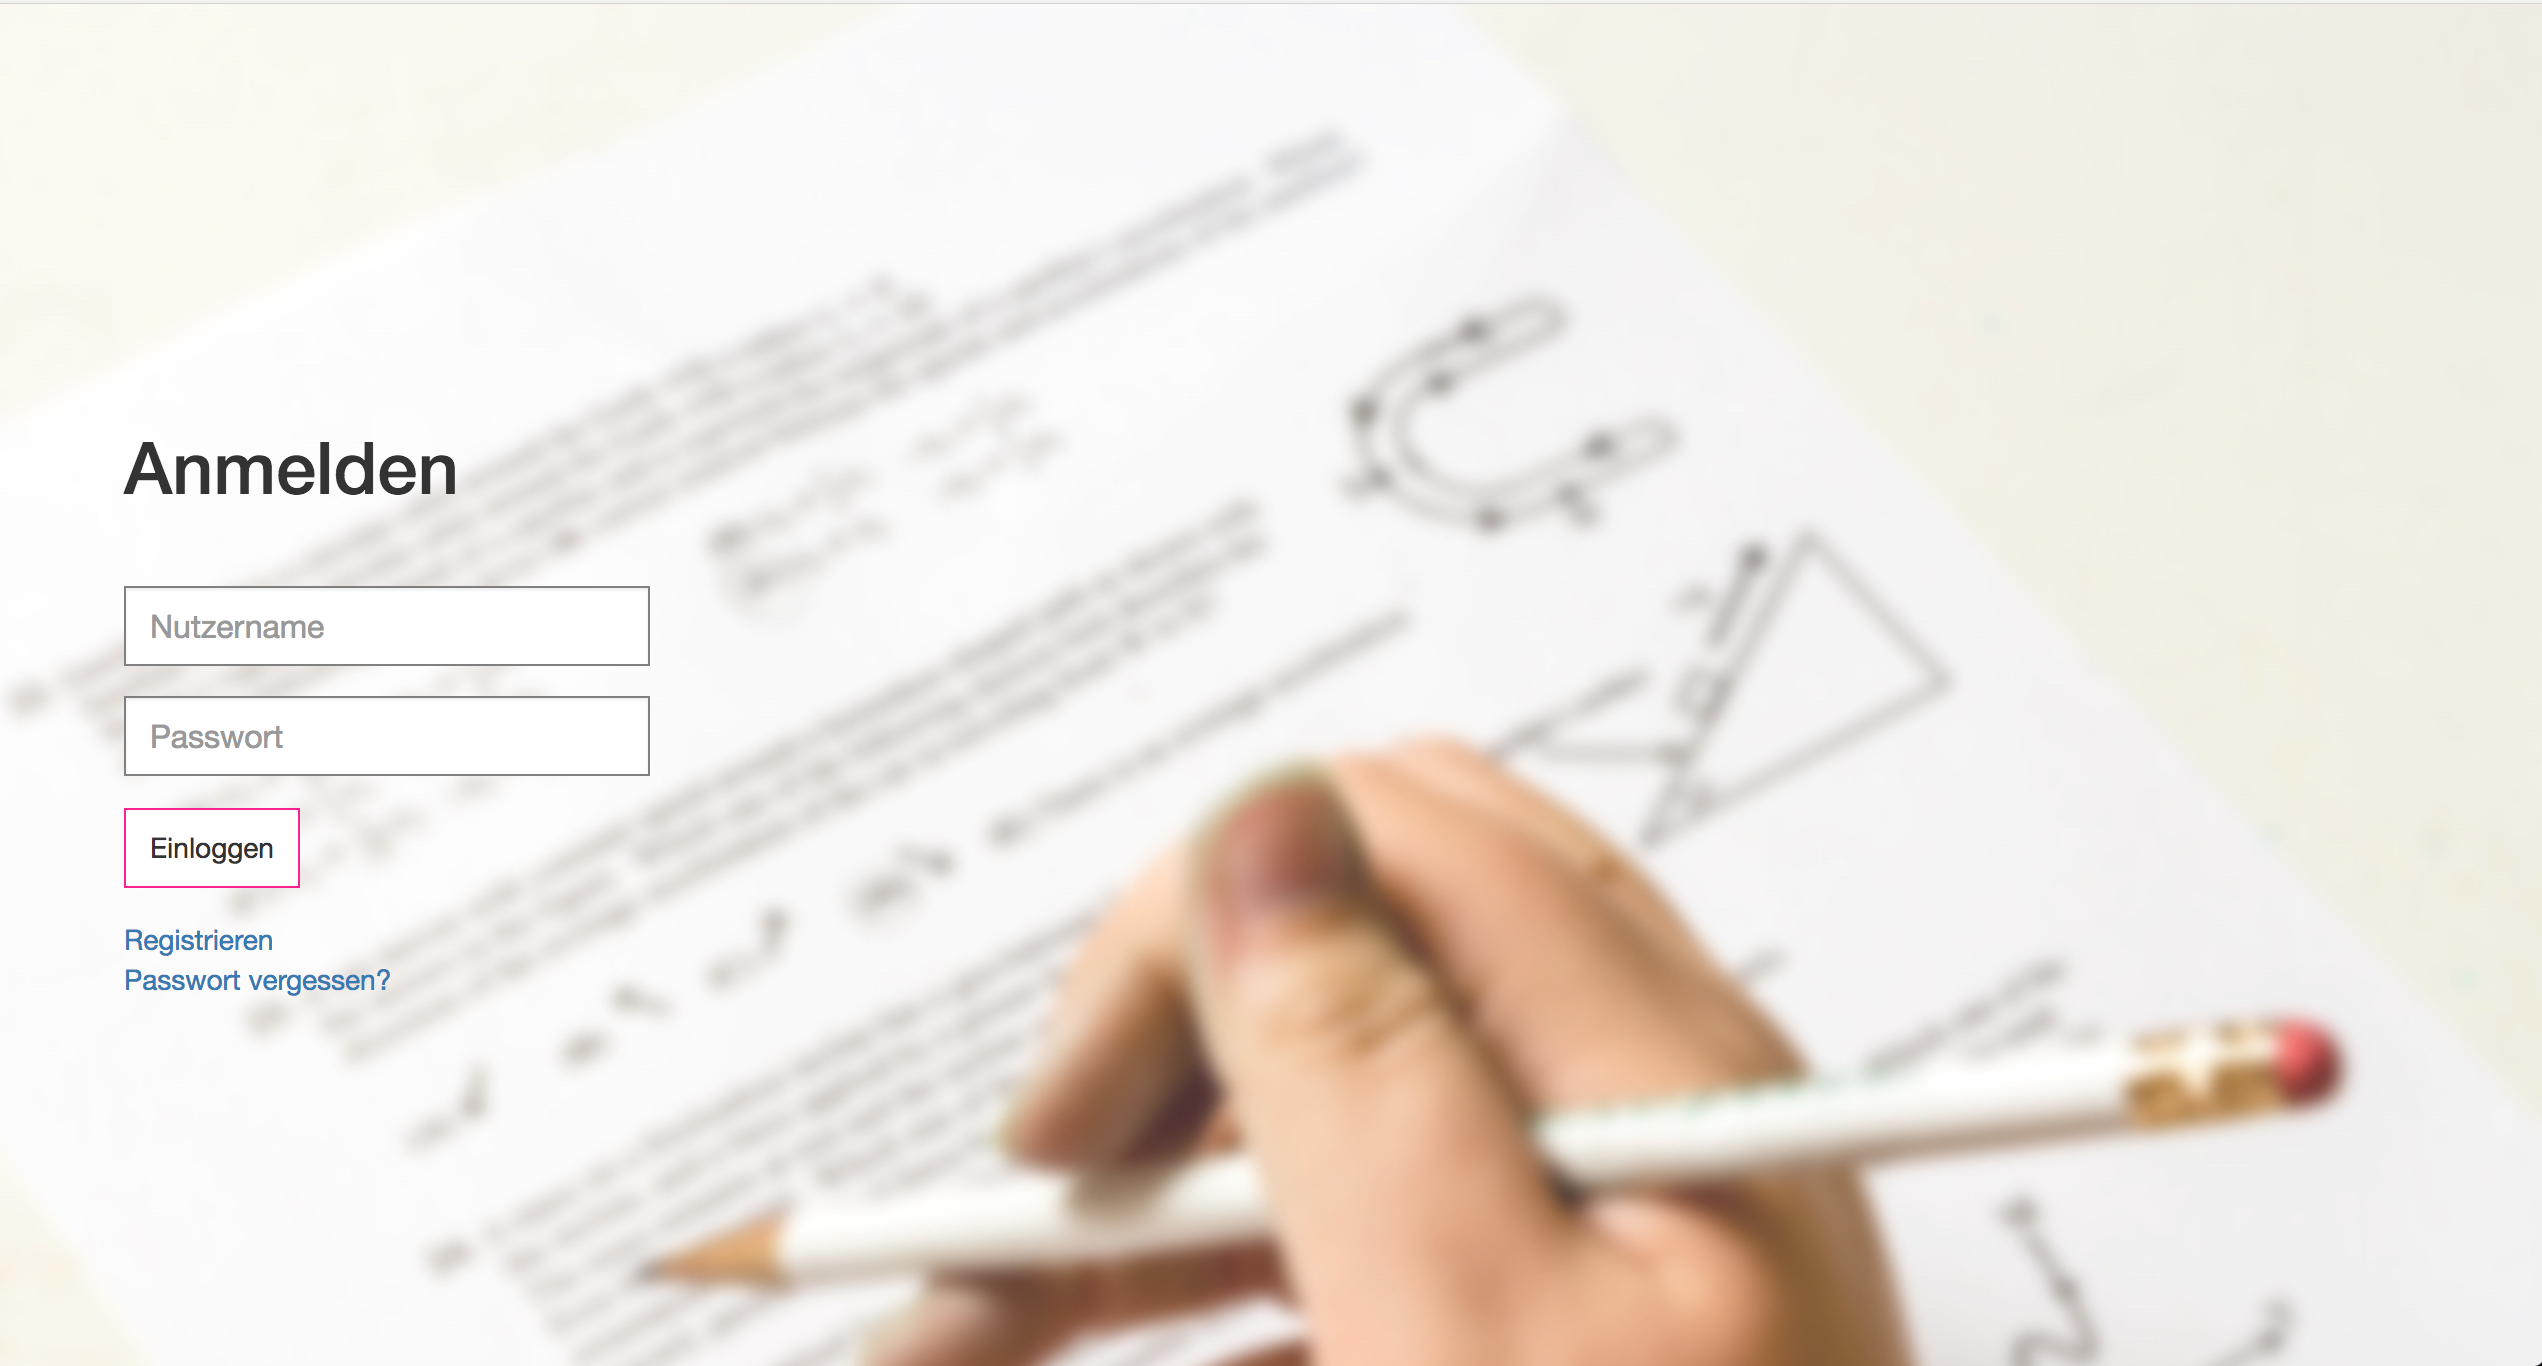
\includegraphics[width=\textwidth,height=10cm,keepaspectratio]{../screenshots/startseite.png}
	\label{fig 1}
\end{figure}

\subsection{Registrierung}
\label{sec:regristrierung}
\subsubsection{Prüfling} 

Nachdem Sie das System Aufgerufen haben und auf der Startseite sind klicken Sie auf Registrieren. Das Registrations-Seite (Abbildung \ref{fig 2})
\begin{figure}[H]
	\centering
	\caption{Registrieren}
  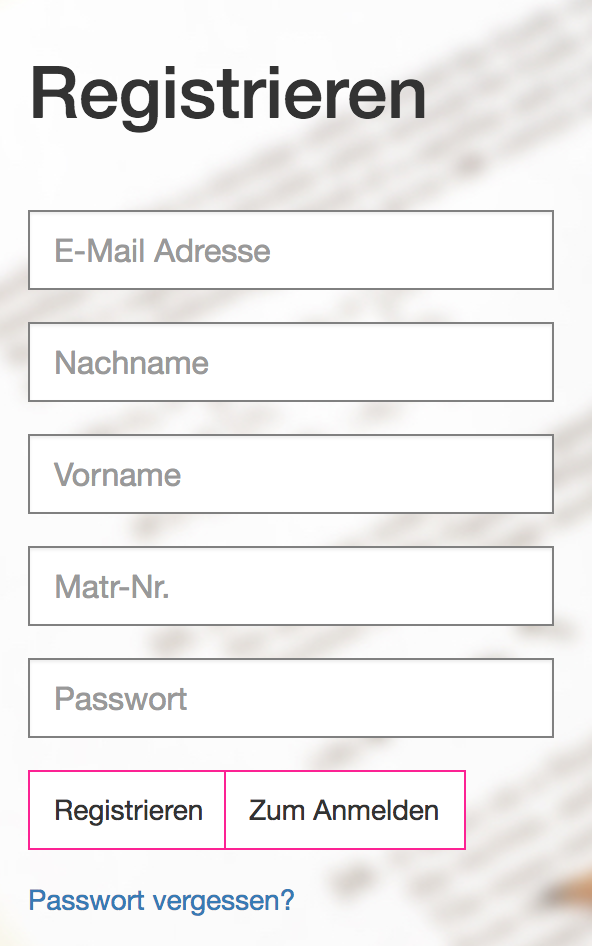
\includegraphics[width=\textwidth,height=10cm,keepaspectratio]{../screenshots/Registrieren/Pruefling/registrieren1.png}
	
	\label{fig 2}
\end{figure}

Füllen Sie die Datenfelder aus. Als E-Mail nutzen Sie Ihre Uni-Mail-Addresse (z.B. ihrname@uni-bremen.de) oder ihr Google-Mail-Adresse und als Passwort das dazugehörige Passwort, so wie Sie sich damit bei Google oder elearning einloggen würden.\\
Wenn Ihre Login-Daten für GoogleMail z.B folgendermaßen aussehen:\\
mail : test@gmail.com\\
passwort: 123\\

So müssen Sie sich bei Grade+ mit genau diesen Daten registrieren.\\
ACHTUNG! Die Matrikelnummer kann später nicht mehr geändert werden, passen Sie auf, das Sie die richtige Matrikelnummer angeben. \\
\\
Wenn Sie alles ausgefüllt haben klicken Sie auf Registrieren. Sie sind jetzt als Nutzer registriert und können sich mit ihrer Uni-Mail-Adresse und Passwort einloggen.


\subsubsection{Admin und Prüfer}
Ein neuer Admin oder Prüfer kann nur von Admins erzeugt werden.\\
Falls Sie sich als Prüfer oder Admin in das System anmelden wollen, kontaktieren Sie bitte einen Admin des Grade+ Systems.\\
Registrieren eines Admins oder Prüfers durch einen Admin wird in {Kapitel \ref{sec:regPuA}} erklärt

\subsection{Login}
Nachdem sich ein Nutzer Registiert hat ({Kapitel \ref{sec:regristrierung}}) kann er/sie sich über die Hauptseite einloggen. Geben Sie dazu Ihre Mail-Adresse und Ihr Passwort an und klicken Sie auf Einloggen.